\section[Introducción]{Introducción}
\subsection[Contexto]{Contexto}
\begin{frame}
    \frametitle{Contexto}
    \begin{columns}
      \column{0.6\textwidth}
    \begin{itemize}
      \item \textbf{La información visual} es cada vez más \textbf{importante}.
        \begin{itemize}
          \item Tanto para el entretenimiento como para el ámbito biomédico.
        \end{itemize}
      \item{Tarea de medir y cuantificar} la calidad perceptual humana de una imagen (IQA). 
        \begin{itemize}
          \item Factores importantes: \textbf{contenido, contraste, distorsiones y la percepción humana}
        \end{itemize}
    \end{itemize}
    \column{0.4\textwidth}
    \begin{figure}
      \begin{center}
        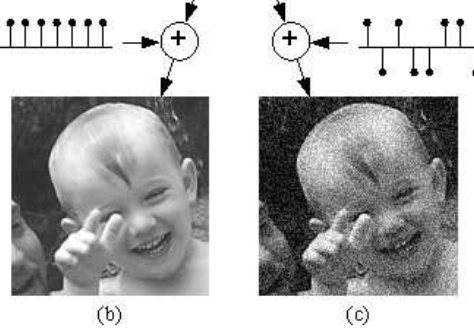
\includegraphics[width=\textwidth]{imagenes/chapter1/failure_minkowski_metricBIG}
      \end{center}
      \caption{Imágenes distorsionadas equidistantes\footnotemark}
    \end{figure}
  \end{columns}
  \vspace{-.2cm}
  \footcitetext{MinkowskiFailure}
\end{frame}

\subsection{Subproblemas}
\begin{frame}
  \frametitle{Estimación con referencia}
  \begin{columns}
  \column{0.5\textwidth}
    \begin{figure}
    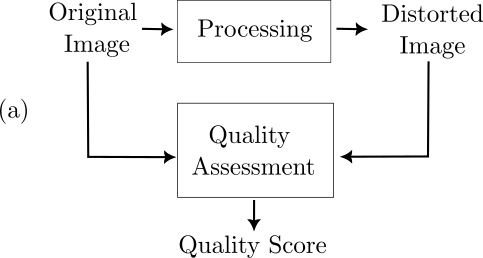
\includegraphics[width=\textwidth]{imagenes/chapter1/FullReferenceInk.png}
    \caption{Problema con referencia (FR).}
    \end{figure}
  \column{0.5\textwidth}
    \begin{figure}
    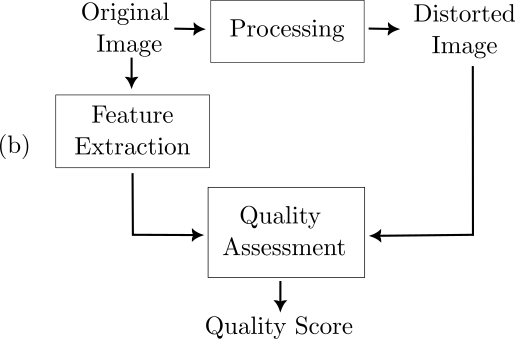
\includegraphics[width=\textwidth]{imagenes/chapter1/ReducedReferenceInk.png}
    \caption{Problema con referencia reducida (RR).}
    \end{figure}
  \end{columns}
\end{frame}

\begin{frame}
  \frametitle{Estimación sin referencia}
  \begin{figure}
    
\includegraphics[width=0.95\textwidth]{imagenes/chapter1/NoReferenceInk.png}
    \caption{Problema sin referencia (NR).}
  \end{figure}
  \begin{enumerate}
    \item El subproblema más \textbf{difícil}.
    \item Debemos disponer de conocimientos sobre: 
      \begin{enumerate}
        \item Naturaleza de las imágenes.
        \item Efecto de las distorsiones.
      \end{enumerate}
    \item \textbf{Este TFG} aborda la estimación, \textbf{sin referencia}, de calidad de imágenes médicas 3D.
  \end{enumerate}
\end{frame}


\subsection{Motivación}
\begin{frame}
  \frametitle{Aplicaciones}
  \begin{columns}
    \column{0.5\textwidth}
  \begin{enumerate}
      \item\textbf{Comparativa} entre algoritmos de compresión.
      \item\textbf{Recuperación} de la información.
      \item\textbf{Evaluar} errores de transmisión.
  \end{enumerate}
  \column{0.5\textwidth}
  \begin{figure}
    \begin{center}
      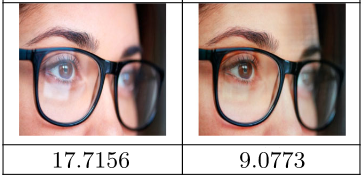
\includegraphics[width=0.85\textwidth]{imagenes/chapter1/Brisque}
    \end{center}
    \caption{
      Eliminación de reflejos en imágenes\footnote[frame]{\cite{BRISQUEExample}}
      con medida de calidad BRISQUE\footnote[frame]{\cite{BRISQUE}}.
  }
  \end{figure}
  \end{columns}
\end{frame}

\begin{frame}
  \frametitle{Motivación}
  \begin{columns}
    \column{0.5\textwidth}
    \begin{itemize}
    \item Cada vez \textbf{más frecuentemente} se emplean volúmenes tridimensionales.
    \item No obstante, las distorsiones \textbf{afectan al volumen 3D generado}. 
    \item Las contribuciones relativas al IQA en la medicina resulta en: 
      \begin{itemize}
        \item Reducción de costes. 
        \item Reducción de tiempo de consulta.
        \item Mejora de calidad del diagnóstico.
      \end{itemize}
    \end{itemize}
  \column{0.5\textwidth}
  \begin{figure}
    \begin{center}
      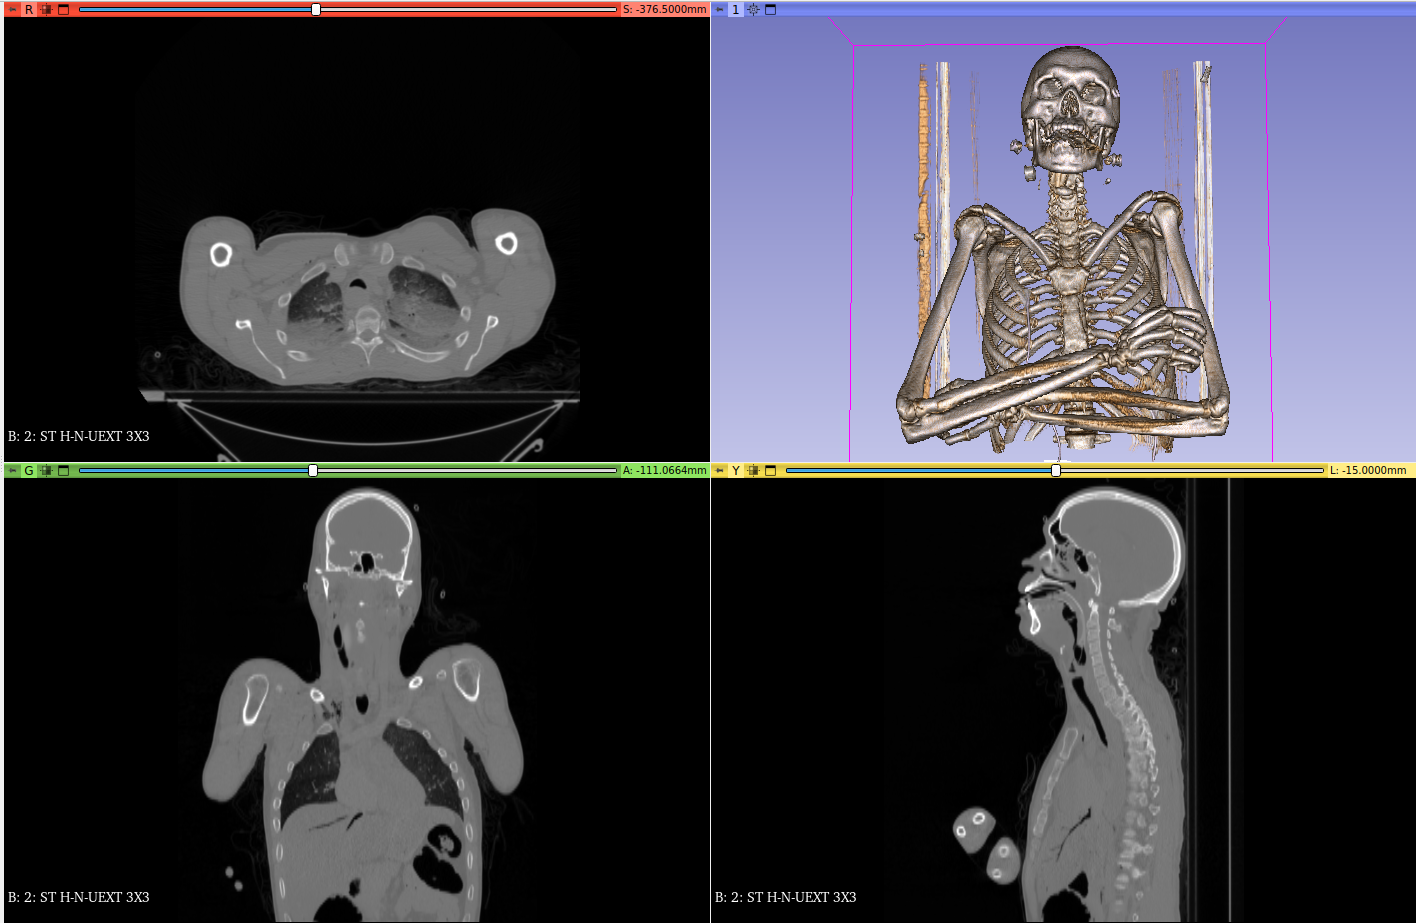
\includegraphics[width=0.95\textwidth]{imagenes/chapter1/SlicerVisualization}
    \end{center}
    \caption{Ejemplo de visualización 3D (Slicer\footnotemark).}
  \end{figure}
  \end{columns}
  \footcitetext{Slicer3D}
\end{frame}


\begin{frame}
  \frametitle{Problemáticas}
  \begin{columns}
    \column{0.5\textwidth}
  \begin{itemize}
    \item El número de métodos propuestos para 3D \textbf{decrece sustancialmente}.
    \item La naturaleza de las imaǵenes médicas \textbf{reduce} la precisión de modelos IQA estándares.
    \item No hay \textbf{ningún} método aplicado \textbf{directamente} a imágenes médicas 3D.
  \end{itemize}
  \column{0.5\textwidth}
  \begin{figure}
    \begin{center}
      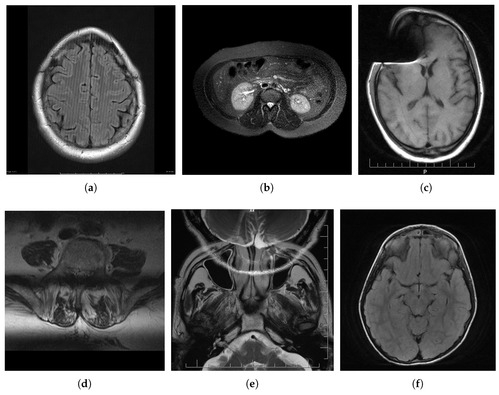
\includegraphics[width=0.78\textwidth]{imagenes/chapter1/MedicalDistortions}
    \end{center}
    \caption{Ejemplo de distorsiones médicas\footnotemark.}
  \end{figure}
  \end{columns}
  \footcitetext{MoreMedicalDistortion}
\end{frame}

\subsection{Objetivos}
\begin{frame}
  \frametitle{Objetivos}
  \begin{columns}

    \column{0.3\textwidth}
  \begin{enumerate}
    \item Estudio exhaustivo del estado del arte. 
    \item Generación de datos sintéticos.
    \item Validar métodos más prometedores.
  \end{enumerate}

  \column{0.7\textwidth}
  \vspace{-.5cm}
  \begin{figure}
      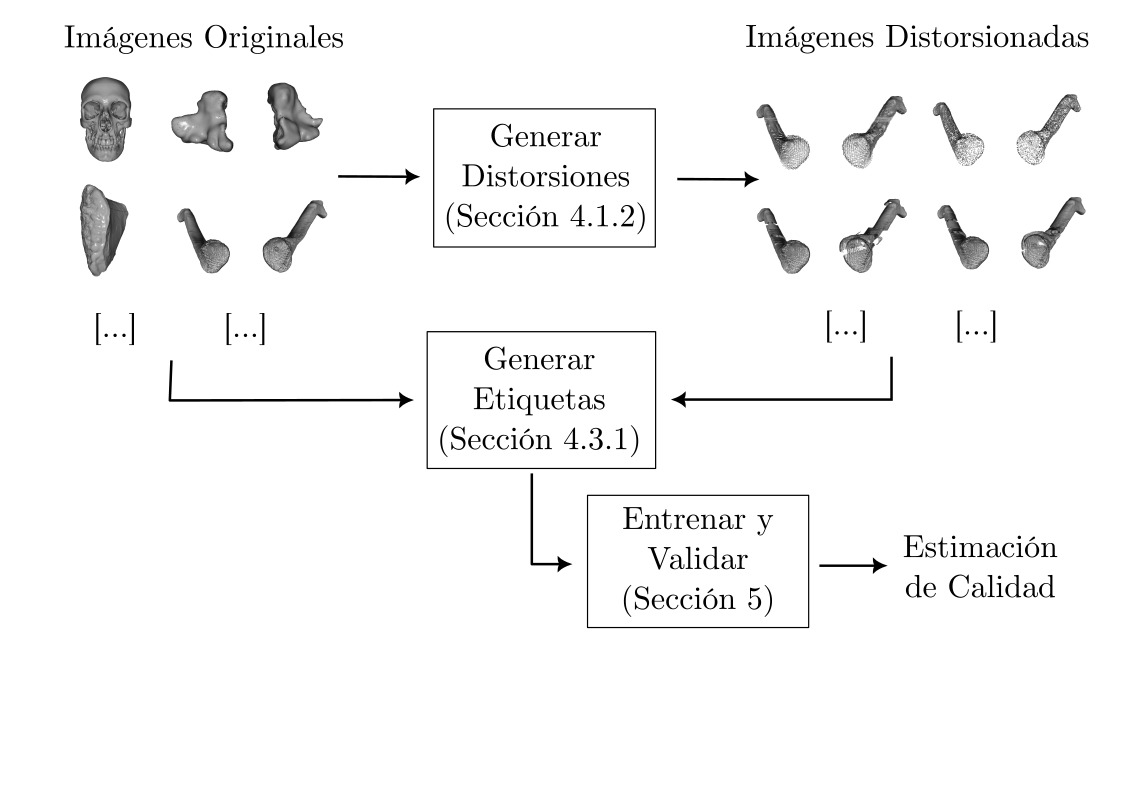
\includegraphics[width=1.0\textwidth, left]{imagenes/chapter1/Objetivos}
  \end{figure}

  \end{columns}
\end{frame}
